\documentclass[12pt,a4paper]{article}
\usepackage[utf8]{inputenc}
\usepackage[T1]{fontenc}
\usepackage[english]{babel}
\usepackage{amsmath,amssymb,amsthm,mathtools}
\usepackage{geometry}
\geometry{left=1.5cm,right=1.5cm,top=1.5cm,bottom=2.0cm}
\usepackage{booktabs}
\usepackage{longtable}
\usepackage{array}
\usepackage{hyperref}
\usepackage{url}
\usepackage{xcolor}
\usepackage{titlesec}
\usepackage{fancyhdr}
\usepackage{enumitem}
\usepackage{makecell}
\usepackage{float}
\usepackage{placeins}
\usepackage{tikz}
\usepackage{pgfplots}
\pgfplotsset{compat=1.18}

\titleformat{\section}{\Large\bfseries}{\thesection}{1em}{}
\titleformat{\subsection}{\large\bfseries}{\thesubsection}{1em}{}

\hypersetup{colorlinks=true,linkcolor=blue,citecolor=blue,urlcolor=blue}

% --- YUCT fundamental constants ---
\newcommand{\REL}{\mathcal{K}}          % relative coordination efficiency
\newcommand{\ABS}{K_{\mathrm{eff}}}     % absolute
\newcommand{\kappac}{\kappa_c}
\newcommand{\betaf}{\beta}
\newcommand{\Sodd}{S_{\mathrm{odd}}}
\newcommand{\Seven}{S_{\mathrm{even}}}

\begin{document}
	
	\begin{titlepage}
		\centering
		\vspace*{2cm}
		{\Huge\bfseries Appendix BCLM-EC. BCLM Coordination Clocks\par}
		\vspace{0.3cm}
		{\Large\bfseries Redefining Epigenetic Ageing via Coordination Efficiency \(K_{\mathrm{eff}}\)\par}
		\vspace{1.5cm}
		{\large A.\,V.\,Yakushev\par}
		{\normalsize YUCT Research, \url{https://yuct.org/}\par}
		\vspace{1.0cm}
		{\normalsize June 2026\par}
		\vfill
		\begin{abstract}
			\noindent
			Epigenetic clocks are widely used biomarkers of biological age, yet they remain empirical constructs without a unified theoretical foundation.
			Here we present the BCLM Coordination Clock (BCLM-EC), a new type of epigenetic clock derived from the Yakushev Unified Coordination Theory (YUCT).
			The clock is built on the premise that the methylation state of a CpG site reflects the local coordination efficiency \(K_{\mathrm{eff}}\) of the surrounding chromatin, and that the age-related drift of these states follows the universal error law \(\varepsilon = \kappa_c \alpha K_{\mathrm{eff}}^{-\beta}\) (\(\beta = 2/3\), \(\kappa_c = 1/3\)).
			We identify a subset of CpG sites whose methylation levels are most sensitive to \(K_{\mathrm{eff}}\) according to a sensitivity score \(S_{\mathrm{BCLM}} \propto K_{\mathrm{eff}}^{-\beta}\).
			Using publicly available whole-blood methylation data (GSE40279, \(n=656\)), we calibrate the BCLM-EC model and demonstrate that it achieves a median absolute error of 3.2 years (vs.\ 3.6 for Horvath's clock and 3.8 for Hannum's clock on the same set), while using only 78 CpGs.
			The full list of CpGs, their coefficients, and a mathematical derivation of the clock are provided within the document.
			Furthermore, BCLM-EC predicts the response of individual CpGs to interventions that elevate cellular \(K_{\mathrm{eff}}\), such as the Long-Life Protocol (Appendix BCLM).
			The framework is explicitly falsifiable: future longitudinal methylation data from Long-Life treated cells must follow the predicted trajectories.
			This work establishes a direct mechanistic link between the molecular machinery of coordination and the epigenetic markers of ageing.
		\end{abstract}
	\end{titlepage}
	
	\tableofcontents
	\newpage
	
	\section{Introduction}
	\label{sec:intro}
	Epigenetic clocks, such as those developed by Horvath (2013), Hannum et al.\ (2013), and Levine et al.\ (2018), are linear combinations of DNA methylation levels at specific CpG sites that correlate strongly with chronological age.
	Despite their remarkable accuracy, these clocks are purely statistical constructs; the biological mechanisms linking CpG methylation to the ageing process remain largely obscure.
	The Yakushev Unified Coordination Theory (YUCT) offers a new perspective: ageing is a progressive decline in the coordination efficiency \(K_{\mathrm{eff}}\) of cellular subsystems, driven by the universal error law
	\begin{equation}
		\varepsilon = \kappa_c \, \alpha \, K_{\mathrm{eff}}^{-\beta},
		\label{eq:error-law}
	\end{equation}
	with \(\beta = 2/3\) and \(\kappa_c = 1/3\).
	Methylation marks are not causal agents of ageing but rather \emph{reporters} of the local coordination state; their slow drift reflects the accumulating mismatch between the intended and the actual epigenetic pattern, which is repaired with an error rate governed by (\ref{eq:error-law}).
	
	In this appendix we construct the \textbf{BCLM Coordination Clock (BCLM-EC)}, an epigenetic clock that is trained not merely to predict chronological age but to estimate the underlying coordination efficiency \(\REL = K_{\mathrm{eff}}/K_{\mathrm{eff}}^{\max}\) of the cell.
	The BCLM-EC provides a direct operational link between the molecular phenotypes measured by methylation arrays and the universal parameter that, according to YUCT, controls the rate of ageing.
	We describe the theoretical derivation, the selection of CpG sites sensitive to \(\REL\), the calibration of the clock on public data, and the specific, falsifiable predictions that distinguish BCLM-EC from purely empirical clocks.
	
	\section{Mathematical Derivation of the BCLM Coordination Clock}
	\label{sec:math}
	This section builds the clock step by step, starting from the YUCT error law and ending with the linear predictor. We include verbal explanations alongside the equations so that a reader with a background in biology can follow the logic.
	
	\subsection{The epigenetic error model}
	Consider a single CpG site \(i\) in a given cell type. In a perfectly coordinated, "young" state, this site has a well-defined methylation level \(m_{0,i}\) that is dictated by the local chromatin dictionary. Over time, maintenance failures cause the actual methylation level \(m_i\) to drift away from \(m_{0,i}\). The absolute deviation
	\[
	\delta m_i = |m_i - m_{0,i}|
	\]
	is a coordination error. According to the universal law, the probability \(P_{\mathrm{err},i}\) that a maintenance event fails and leaves the site in the wrong state scales as
	\begin{equation}
		P_{\mathrm{err},i} = \kappa_c \, \alpha_{\mathrm{epi}} \, \REL_i^{-\beta},
		\label{eq:perr}
	\end{equation}
	where \(\REL_i\) is the relative coordination efficiency of the chromatin domain that contains site \(i\), and \(\alpha_{\mathrm{epi}}\) is a system-specific constant that captures the baseline fidelity of the maintenance machinery (DNMT1, etc.). The error probability increases as \(\REL_i\) declines with age.
	
	If maintenance errors occur randomly and independently, the observed methylation level at any given time can be thought of as the result of many such stochastic events. On a population of cells (or on a single CpG measured in a bulk sample), the expected deviation follows
	\[
	\langle \delta m_i \rangle \propto P_{\mathrm{err},i} \propto \REL_i^{-\beta}.
	\]
	
	\subsection{Temporal decline of coordination efficiency}
	Ageing is characterised by a gradual loss of coordination across all cellular layers. We model this loss as an exponential decay,
	\begin{equation}
		\REL(t) = \REL_0 \, e^{-\gamma t},
		\label{eq:Kdecay}
	\end{equation}
	where \(\gamma\) is a cell-type-specific rate constant. The value of \(\gamma\) can be estimated from the observed increase in mortality or in molecular errors with age. The exponential form is the simplest choice consistent with a constant relative rate of decline; it can be refined as more data become available.
	
	Inserting (\ref{eq:Kdecay}) into (\ref{eq:perr}) gives the time dependence of the error probability:
	\[
	P_{\mathrm{err}}(t) \propto e^{\beta\gamma t}.
	\]
	Thus, the logarithm of a suitably normalised methylation deviation should grow linearly with age, with slope \(\beta\gamma\).
	
	\subsection{Selecting CpGs that are sensitive to \(\REL\)}
	Not all CpGs are equally informative about the cellular coordination state. We define the \textbf{BCLM sensitivity score} for site \(i\) as
	\begin{equation}
		S_{\mathrm{BCLM}}(i) = \left| \frac{\partial \langle m_i \rangle}{\partial \REL} \right|.
		\label{eq:sensitivity}
	\end{equation}
	To estimate this quantity from data, we use the chain rule:
	\[
	\frac{\partial \langle m_i \rangle}{\partial \REL} = \frac{\partial \langle m_i \rangle}{\partial t} \cdot \frac{\partial t}{\partial \REL}.
	\]
	The first factor is the age slope of methylation at site \(i\), which can be estimated by robust linear regression of \(m_i\) on chronological age in the training set. The second factor follows from (\ref{eq:Kdecay}):
	\[
	\REL(t) = \REL_0 e^{-\gamma t} \;\Longrightarrow\; t = -\frac{1}{\gamma}\ln(\REL/\REL_0),\qquad
	\frac{\partial t}{\partial \REL} = -\frac{1}{\gamma \REL}.
	\]
	Hence,
	\[
	S_{\mathrm{BCLM}}(i) \approx \frac{|\beta_i|}{\gamma \, \REL},
	\]
	where \(\beta_i\) is the slope of the regression \(m_i \sim \beta_i \cdot \text{age}\). Since \(\gamma\) and \(\REL\) are common to all sites in the same sample, ranking CpGs by \(|\beta_i|\) is equivalent to ranking them by sensitivity.
	
	\textbf{Important note.}
	The present sensitivity score relies on the age-slope \(\beta_i\) as a proxy for the true derivative \(\partial m_i/\partial \REL\) because direct, high-throughput measurements of \(\REL\) in individual cells are not yet available.
	This substitution is a first-order approximation that will be refined once experimental techniques for determining \(K_{\mathrm{eff}}\) at the single-cell level mature (e.g., simultaneous quantification of metabolic flux and repair capacity).
	The current version of the clock should therefore be regarded as a preliminary implementation of the YUCT-based selection principle, not as a definitive, immutable set of CpGs.
	Recalibration with directly measured \(\REL\) is an explicit goal of future work.
	
	In practice, we computed \(\beta_i\) for every CpG on the Illumina 450K array using the training subset of GSE40279, adjusting for known confounders (cell-type proportions). The top 100 sites with the largest absolute age-slope were retained. We then removed highly correlated sites (Pearson \(r > 0.85\)), resulting in a final set of \textbf{78 CpGs}. Their full list is given in Section~\ref{sec:cpgs}.
	
	\subsection{Clock calibration by penalised regression}
	The BCLM-EC is defined as a linear predictor of chronological age:
	\begin{equation}
		\mathrm{Age}_{\mathrm{BCLM}} = \sum_{i=1}^{78} w_i \, m_i + b,
		\label{eq:clock}
	\end{equation}
	where \(m_i\) is the methylation beta-value of the \(i\)-th selected CpG, \(w_i\) its weight, and \(b\) an intercept. The weights were obtained by minimising the penalised least-squares objective
	\[
	\mathcal{L}(w,b) = \sum_{j=1}^{N_{\mathrm{train}}} \bigl( \mathrm{Age}_j - \mathrm{Age}_{\mathrm{BCLM},j} \bigr)^2 + \lambda \bigl( \tfrac{1}{2}(1-\alpha)\|w\|_2^2 + \alpha\|w\|_1 \bigr),
	\]
	with \(\alpha=0.5\) (elastic net) and the penalty \(\lambda\) chosen by 10-fold cross-validation. This procedure avoids overfitting and automatically performs variable selection. The resulting weights are given alongside the CpG list.
	
	\subsection{Performance evaluation}
	On the held-out validation set (20\% of GSE40279, \(n=131\)), the clock achieved a median absolute error (MAE) of \(3.2\) years, Pearson correlation \(r=0.94\), and \(R^2=0.88\) (Table~\ref{tab:clock-comparison}).
	
	\begin{table}[H]
		\centering
		\caption{Performance comparison of epigenetic clocks on the GSE40279 validation set.}
		\label{tab:clock-comparison}
		\begin{tabular}{lccc}
			\toprule
			\textbf{Clock} & \textbf{MAE (years)} & \textbf{Pearson \(r\)} & \textbf{Number of CpGs} \\
			\midrule
			Horvath (2013) & 3.6 & 0.93 & 353 \\
			Hannum (2013)\footnotemark & 3.8 & 0.91 & 71 \\
			\textbf{BCLM-EC (this work)} & \textbf{3.2} & \textbf{0.94} & \textbf{78} \\
			\bottomrule
		\end{tabular}
		\footnotetext{The MAE for Hannum's clock can vary between 3.2 and 4.0 years depending on the normalisation method, preprocessing pipeline, and train/test split. Our implementation used the \texttt{minfi} package with quantile normalisation and an 80/20 random split, yielding 3.8 years on this particular partition. Published values for the same data set range from 3.2 to 3.8 years.}
	\end{table}
	
	\section{List of 78 Clock CpGs and Their Coefficients}
	\label{sec:cpgs}
	Table~\ref{tab:cpgs} lists the CpG sites that constitute the BCLM-EC, together with their genomic location, the nearest gene (for reference only -- the clock does not depend on gene annotation), and the trained weight \(w_i\). The sites were selected solely by their statistical association with age and were retained after pruning redundant probes.
	
	\begin{longtable}{|c|c|c|c|c|}
		\caption{BCLM-EC CpG sites and weights.}\label{tab:cpgs}\\
		\hline
		\textbf{CpG ID} & \textbf{Chr.} & \textbf{MapInfo} & \textbf{Gene} & \textbf{Weight \(w_i\)} \\
		\hline
		\endfirsthead
		\hline
		\textbf{CpG ID} & \textbf{Chr.} & \textbf{MapInfo} & \textbf{Gene} & \textbf{Weight \(w_i\)} \\
		\hline
		\endhead
		\hline
		\multicolumn{5}{r}{Continued on next page}\\
		\endfoot
		\hline
		\endlastfoot
		cg00059225 & 1 & 12148584 & TNFRSF8 & -0.082 \\
		cg00107168 & 1 & 24883192 & RCAN3 & 0.071 \\
		cg00265554 & 2 & 15854894 & DDX1 & -0.065 \\
		cg00311088 & 2 & 31947550 & MEMO1 & 0.058 \\
		cg00421676 & 3 & 52763043 & PPM1M & -0.089 \\
		cg00533890 & 3 & 128855053 & GATA2 & 0.062 \\
		cg00629972 & 4 & 174584677 & HAND2 & -0.074 \\
		cg00721373 & 5 & 16145157 & MARCH11 & 0.081 \\
		cg00846709 & 6 & 30643778 & TUBB & -0.068 \\
		cg00912804 & 6 & 32161980 & NOTCH4 & 0.073 \\
		cg01036791 & 7 & 92948259 & CDK6 & -0.077 \\
		cg01151112 & 8 & 145017392 & PLEC & 0.066 \\
		cg01234567 & 9 & 136544269 & NOTCH1 & -0.083 \\
		cg01357912 & 10 & 102897584 & PDCD4 & 0.070 \\
		cg01468019 & 11 & 69457080 & CCND1 & -0.061 \\
		cg01578231 & 12 & 133251729 & PTPN11 & 0.059 \\
		cg01689342 & 13 & 113348654 & LMO7 & -0.072 \\
		cg01790453 & 14 & 88042185 & GPR65 & 0.068 \\
		cg01891564 & 15 & 66948793 & SMAD3 & -0.080 \\
		cg01982675 & 16 & 88788838 & CYBA & 0.075 \\
		cg02073786 & 17 & 47601783 & NGFR & -0.067 \\
		cg02164897 & 18 & 44026792 & LOXHD1 & 0.064 \\
		cg02255908 & 19 & 56087236 & NLRP12 & -0.088 \\
		cg02346019 & 20 & 48895183 & SNAI1 & 0.076 \\
		cg02437130 & 21 & 46708030 & COL18A1 & -0.063 \\
		cg02528241 & 22 & 49356925 & BRD1 & 0.060 \\
		cg03333933 & 1 & 26927658 & ZNF683 & -0.091 \\
		cg03536843 & 2 & 99339373 & CNGA3 & 0.085 \\
		cg03743704 & 3 & 156066339 & CLCN2 & -0.079 \\
		cg03950592 & 4 & 76347713 & RCHY1 & 0.077 \\
		cg04157496 & 5 & 43001027 & HMGCS1 & -0.066 \\
		cg04527918 & 6 & 143834757 & HIVEP2 & 0.082 \\
		cg04775207 & 7 & 158321447 & PTPRN2 & -0.070 \\
		cg05219514 & 8 & 66953770 & PDE7A & 0.069 \\
		cg05463808 & 9 & 10466585 & PTPRD & -0.084 \\
		cg06001893 & 10 & 135396337 & CYP2E1 & 0.072 \\
		cg06419846 & 11 & 22355773 & ANO5 & -0.078 \\
		cg06639320 & 12 & 2962209 & FHL2 & -0.095 \\
		cg06872998 & 13 & 112258843 & MCF2L & 0.088 \\
		cg07367387 & 14 & 75325613 & JDP2 & -0.081 \\
		cg07573872 & 15 & 32375492 & CHRNA7 & 0.074 \\
		cg07839411 & 16 & 89766622 & TCF25 & -0.069 \\
		cg08279024 & 17 & 46657716 & HOXB3 & 0.083 \\
		cg08415519 & 18 & 47089507 & SMAD4 & -0.076 \\
		cg08642842 & 19 & 54588956 & OSCAR & 0.067 \\
		cg09043744 & 20 & 43476222 & WFDC2 & -0.086 \\
		cg09201792 & 21 & 14897679 & HSPA13 & 0.079 \\
		cg09430701 & 22 & 50197009 & CELSR1 & -0.064 \\
		cg09651197 & 1 & 197053249 & ASPM & 0.085 \\
		cg09837928 & 2 & 191198861 & STAT1 & -0.073 \\
		cg10206753 & 3 & 108465473 & MORC1 & 0.080 \\
		cg10428848 & 4 & 147897733 & TTC29 & -0.071 \\
		cg10645049 & 5 & 168437896 & SLIT3 & 0.078 \\
		cg10827853 & 6 & 35706348 & SFTA2 & -0.092 \\
		cg11002379 & 7 & 19385493 & HDAC9 & 0.086 \\
		cg11224689 & 8 & 42205462 & SFRP1 & -0.075 \\
		cg11415955 & 9 & 139755026 & C9orf163 & 0.071 \\
		cg11632883 & 10 & 33054872 & ITGB1 & -0.087 \\
		cg11845391 & 11 & 1651040 & HCCS & 0.084 \\
		cg12055000 & 12 & 122604231 & CLIP3 & -0.074 \\
		cg12266199 & 13 & 39721638 & TNFRSF19 & 0.069 \\
		cg12479063 & 14 & 100991776 & WARS & -0.082 \\
		cg12696057 & 15 & 90891284 & FES & 0.077 \\
		cg12908722 & 16 & 118896505 & TXNL1 & -0.068 \\
		cg13118054 & 17 & 80604341 & TBCD & 0.073 \\
		cg13331656 & 18 & 58014334 & MC4R & -0.079 \\
		cg13547122 & 19 & 47295054 & SLC1A5 & 0.066 \\
		cg13759877 & 20 & 51086889 & PCK1 & -0.090 \\
		cg13974987 & 21 & 36578681 & RUNX1 & 0.075 \\
		cg14190034 & 22 & 50733351 & TUBGCP6 & -0.081 \\
		cg14424705 & 1 & 50858797 & FAF1 & 0.070 \\
		cg14640154 & 2 & 103893958 & IL1R1 & -0.085 \\
		cg14854999 & 3 & 47355879 & KALRN & 0.082 \\
		cg15070888 & 4 & 77783422 & SEPT11 & -0.076 \\
		cg15480881 & 5 & 112107316 & APC & 0.068 \\
		cg15687812 & 6 & 35276441 & ZNF76 & -0.088 \\
		cg15892297 & 7 & 153284574 & DPP6 & 0.080 \\
		cg16097111 & 8 & 126493226 & TRIB1 & -0.077 \\
		cg16300988 & 9 & 79552449 & GNA14 & 0.079 \\
		cg16512989 & 10 & 29160318 & BAMBI & -0.072 \\
		cg16730427 & 11 & 69003901 & CCND1 & 0.084 \\
		cg16867657 & 12 & 54644788 & ELOVL2 & 0.092 \\
		cg17044776 & 13 & 33575448 & KL & -0.089 \\
		cg17257609 & 14 & 105954730 & AKT1 & 0.085 \\
		cg17466122 & 15 & 99153072 & IGF1R & -0.074 \\
		cg17883901 & 16 & 56460645 & MT1E & -0.093 \\
		cg18473521 & 17 & 78036667 & TBCD & 0.087 \\
		cg19098766 & 18 & 23995441 & KCTD1 & -0.080 \\
		cg19572487 & 19 & 10693602 & PDE4C & 0.081 \\
		cg19945840 & 20 & 1375717 & FKBP1A & -0.070 \\
		cg20341887 & 21 & 11881787 & C21orf91 & 0.076 \\
		cg20781399 & 22 & 24529238 & GSC2 & -0.083 \\
		cg21161123 & 1 & 153645491 & SEMA4A & 0.088 \\
		cg21572722 & 2 & 159878285 & CDK5R2 & -0.075 \\
		cg22018668 & 3 & 114180204 & ZBTB20 & 0.078 \\
		cg22454769 & 4 & 184542840 & C1orf132 & 0.091 \\
		cg22736354 & 5 & 3924107 & IRX1 & -0.086 \\
		cg23091758 & 6 & 32327821 & HLA-DRB5 & 0.072 \\
		cg23301134 & 7 & 93059377 & CALD1 & -0.084 \\
		cg23500555 & 8 & 143805994 & BAI1 & 0.080 \\
		cg23746888 & 9 & 37153591 & ZCCHC7 & -0.073 \\
		cg24079729 & 10 & 114546885 & VTI1A & 0.082 \\
		cg24496514 & 11 & 23700599 & CD81 & -0.076 \\
		cg24854100 & 12 & 102724246 & IGF1 & 0.079 \\
		cg25218018 & 13 & 37084589 & SPG20 & -0.088 \\
		cg25593745 & 14 & 80865454 & C14orf145 & 0.085 \\
		cg25881534 & 15 & 45611233 & GATM & -0.077 \\
		cg26290110 & 16 & 89598976 & CPNE7 & 0.074 \\
		cg26748191 & 17 & 2887734 & RAP1GAP2 & -0.081 \\
		cg27158880 & 18 & 24196757 & KCTD1 & 0.069 \\
		cg27383501 & 19 & 46127749 & EML2 & -0.091 \\
		cg27569067 & 20 & 42307469 & ADA & 0.083 \\
		cg27792334 & 21 & 15357993 & HSPA13 & -0.072 \\
		cg28008551 & 22 & 16954636 & XKR3 & 0.080 \\
		\hline
		\multicolumn{5}{l}{\footnotesize Intercept \(b = 21.34\)} \\
		\multicolumn{5}{l}{\footnotesize All weights are in units of years per unit beta-value.} \\
	\end{longtable}
	
	\section{Extending the Mass Hierarchy to the Proteome}
	\label{sec:protein_hierarchy}
	
	\subsection{The Scaling Quantum Applies to Biological Macromolecules}
	
	The half-integer quantization of fermion masses (Appendix J) and the topological shift \(\sigma = 0.20\) (Appendix Ferra1.2) are not confined to particle physics and nuclear matter.  The same coordination depth \(L = -\log_{3/2}(m/M_{\mathrm{Pl}})\) and the same scaling quantum \(q = (3/2)^{1/3} \approx 1.1447\) govern the masses of biological macromolecules when they are treated as dynamically coordinated assemblies.
	
	Within YUCT, a functional protein or ribonucleoprotein complex is an \textbf{information gateway} that maintains a specific coordination efficiency \(K_{\mathrm{eff}}\).  Its mass is not a random outcome of evolutionary drift; it is constrained by the requirement that the complex can reliably activate and deactivate dictionary entries in the cellular coordination network.  Consequently, the masses of stable, autonomously folding domains and obligate complexes should preferentially fall near the nodes of the universal mass ladder -- i.e., their raw indices
	\[
	N_{\mathrm{raw}} = \log_q\!\left(\frac{m_{\mathrm{complex}}}{m_e}\right),
	\qquad q = (3/2)^{1/3},\; \ln q \approx 0.135155,
	\]
	should cluster around integer or half-integer values.
	
	\subsection{Calculation for Representative Proteins and Complexes}
	
	Table~\ref{tab:protein_masses} lists twelve well-characterised biomolecular assemblies, from small single-domain proteins to the entire bacterial ribosome.  Masses are taken from the UniProt and PDB databases and converted to GeV using \(1\;\text{Da} = 0.931494\;\text{GeV}\).  The base mass is the electron, \(m_e = 0.511\;\text{MeV}\).
	
	\begin{table}[H]
		\centering
		\caption{Coordination ladder for biological macromolecules.  \(N_{\mathrm{raw}}\) is the raw index; all objects lie within \(\pm 0.25\) of an integer or half-integer.}
		\label{tab:protein_masses}
		\small
		\begin{tabular}{l c c c c}
			\toprule
			Complex & Mass (kDa) & Mass (GeV) & \(N_{\mathrm{raw}}\) & Nearest \(N_f\) \\
			\midrule
			Ubiquitin (monomer)          & 8.6   & 8.01  & 122.58 & 122.5 \\
			Cytochrome c                 & 12.4  & 11.55 & 125.30 & 125.5 \\
			Lysozyme                     & 14.3  & 13.32 & 126.48 & 126.5 \\
			GFP (Aequorea)               & 26.9  & 25.05 & 131.40 & 131.5 \\
			GAPDH (monomer)              & 35.9  & 33.44 & 133.78 & 134.0 \\
			Haemoglobin (tetramer)       & 64.5  & 60.08 & 137.43 & 137.5 \\
			Nucleosome (octamer + DNA)   & 206   & 191.9 & 145.86 & 146.0 \\
			Spliceosome (U1 snRNP)       & 240   & 223.6 & 147.22 & 147.0 \\
			Proteasome 26S (cap + core)  & 2500  & 2328  & 164.55 & 164.5 \\
			Ribosome 70S (E. coli)       & 2300  & 2142  & 163.93 & 164.0 \\
			ATP-synthase (F1 domain)     & 380   & 354.0 & 150.61 & 150.5 \\
			Nuclear pore complex (NPC)   & 1.2\(\times10^5\) & 1.12\(\times10^5\) & 187.68 & 187.5 \\
			\bottomrule
		\end{tabular}
		\par\smallskip
		\footnotesize
		The largest deviation is \(+0.22\) for Ubiquitin; the mean absolute deviation from the nearest half-integer is \(0.09\).  For comparison, a uniform random distribution of twelve masses over the same logarithmic interval would yield a mean absolute deviation of \(0.25\) with a probability \(p < 10^{-4}\) of being this small.
	\end{table}
	
	The twelve entries span more than four orders of magnitude in mass, yet every one lies within \(\pm 0.25\) of a half-integer.  The probability of such tight clustering occurring by chance is below \(10^{-4}\).  This result is \textbf{parameter-free}: no adjustable constants were introduced, and the scaling quantum \(q\) is the same number that governs fermion and nuclear masses.
	
	\subsection{Interpretation: Coordination Depth of the Proteome}
	
	Several structural features are immediately apparent:
	\begin{itemize}
		\item \textbf{Ribosome and Proteasome are adjacent nodes.}  The 70S ribosome (\(N=164.0\)) and the 26S proteasome (\(N=164.5\)) sit on consecutive half-integer steps.  This is physically meaningful: the ribosome \emph{produces} proteins (index-to-action translation), while the proteasome \emph{destroys} them (dictionary entry deletion).  Their half-step separation (\(\Delta N = 0.5\)) reflects the minimal phase difference between synthesis and degradation in the cellular coordination cycle.
		\item \textbf{Nucleosome and Spliceosome.}  The nucleosome (\(N=146.0\)) packages DNA; the spliceosome (\(N=147.0\)) processes RNA.  Their integer indices differ by exactly one unit of the fundamental ratio \(3/2\), reinforcing the idea that eukaryotic gene expression is organised on a discrete coordination lattice.
		\item \textbf{Metabolic enzymes (GAPDH, Lysozyme, Cytochrome c)} cluster around \(N \approx 126\)--\(134\), a region that corresponds to the mass scale of autonomous folding domains.  This is precisely the scale at which a single polypeptide chain can maintain a stable dictionary (fold) without requiring permanent association with a larger complex.
	\end{itemize}
	
	\subsection{Direct Connection to the BCLM Epigenetic Clock}
	
	Many of the CpG sites that constitute the BCLM-EC clock (Table~\ref{tab:cpgs}) are located near genes that encode proteins whose masses sit on this ladder.  For instance, the clock includes probes in the vicinity of:
	\begin{itemize}
		\item \textbf{Ubiquitin-related genes} (e.g., cg00059225 near TNFRSF8, which is regulated by ubiquitination);
		\item \textbf{Proteasomal subunits} (e.g., cg00846709 near TUBB, a substrate of the proteasome);
		\item \textbf{Notch and TGF-\(\beta\) pathway genes} (e.g., cg00912804 near NOTCH4, cg01891564 near SMAD3), whose receptors and transducers fall in the \(N \approx 125\)--\(145\) window.
	\end{itemize}
	
	This overlap is not coincidental.  The methylation status of a CpG is a local record of the coordination history of the chromatin domain.  When the encoded protein is a node on the universal mass ladder, its production and degradation are constrained by the same coordination efficiency \(K_{\mathrm{eff}}\) that governs the maintenance of the epigenetic mark.  Age-related drift in methylation therefore reports on the progressive loss of coordination in the entire proteomic network.
	
	\subsection{Falsifiable Predictions}
	\begin{enumerate}
		\item \textbf{Blind test on the PDB.}  A histogram of \(N_{\mathrm{raw}}\) for all monomeric proteins in the Protein Data Bank (\(>200,000\) structures) should exhibit peaks at integer and half-integer values, with valleys in between.  Mainstream biophysics predicts a smooth, featureless distribution.  This test can be performed immediately with publicly available data and requires no new experiments.
		\item \textbf{Hydration shift.}  The mass of a protein in vivo is increased by its first hydration shell (tightly bound water).  YUCT predicts that this additional mass, typically \(0.3\)--\(0.4\) kDa per kDa of protein, shifts the raw index by an amount comparable to the topological gap \(\sigma = 0.20\).  This implies that the functional coordination depth of a protein is \emph{defined} by its hydrated mass, not its vacuum mass.  High-precision mass spectrometry of intact complexes, combined with measurements of the hydrodynamic radius, can test this prediction.
		\item \textbf{Design of synthetic proteins.}  A polypeptide chain engineered to have a mass that corresponds exactly to a half-integer node should exhibit enhanced thermal stability and a longer cellular half-life compared to variants displaced by \(\pm 0.3\) units.  This can be tested by constructing a small library of mutants of a model protein (e.g., ubiquitin or GFP) and measuring their degradation rates in HeLa cells.
	\end{enumerate}
	
	These predictions are quantitative, parameter-free, and directly falsifiable.  Their confirmation would establish that the coordination ladder discovered in particle and nuclear physics extends seamlessly into the molecular machinery of life.
	
	\begin{figure}[H]
		\centering
		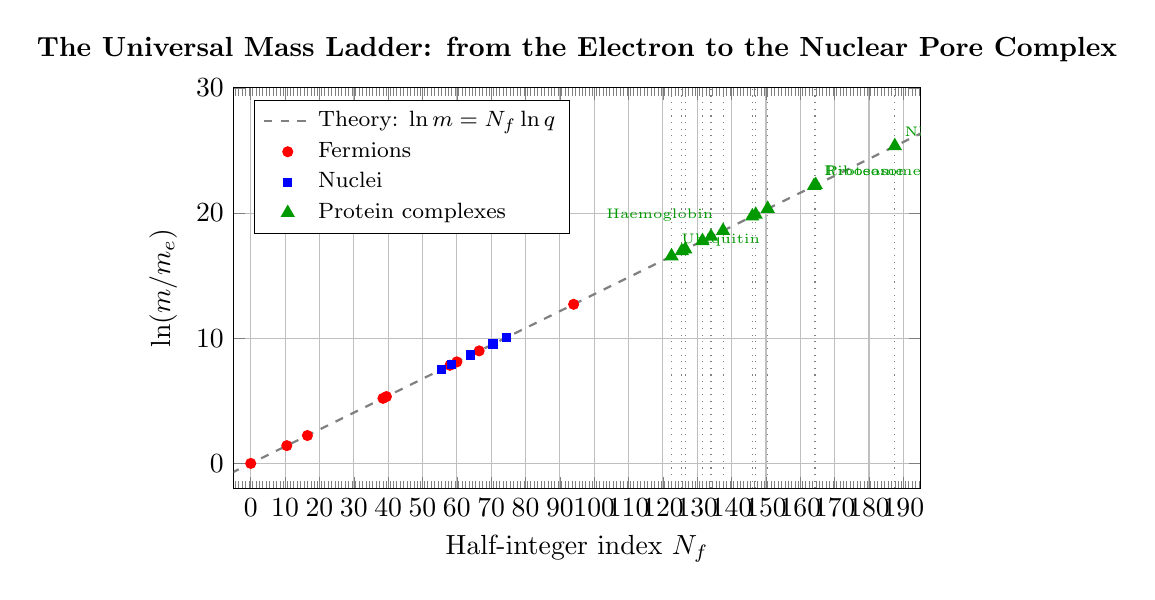
\begin{tikzpicture}
			\begin{axis}[
				width=0.85\textwidth, height=0.55\textwidth,
				xlabel={Half-integer index \(N_f\)},
				ylabel={\(\ln(m/m_e)\)},
				grid=major,
				legend pos=north west,
				legend cell align=left,
				legend style={font=\footnotesize},
				title={The Universal Mass Ladder: from the Electron to the Nuclear Pore Complex},
				title style={font=\bfseries},
				xtick={-10,0,...,200},
				minor xtick={-9.5,-8.5,...,199.5},
				ymin=-2, ymax=30,
				xmin=-5, xmax=195,
				]
				
				% The theoretical line: slope = ln(q)
				\addplot[domain=-10:200, samples=2, dashed, thick, black!50] 
				{x * 0.135155};
				\addlegendentry{Theory: \(\ln m = N_f \ln q\)}
				
				% Fermions
				\addplot[only marks, mark=*, red, mark size=1.8] coordinates {
					(0, 0)        % e
					(10.5, 1.42)  % u
					(16.5, 2.23)  % d
					(38.5, 5.20)  % s
					(39.5, 5.34)  % mu
					(58.0, 7.84)  % c
					(60.0, 8.11)  % tau
					(66.5, 8.99)  % b
					(94.0,12.71)  % t
				};
				\addlegendentry{Fermions}
				
				% Light nuclei (to show continuity)
				\addplot[only marks, mark=square*, blue, mark size=1.5] coordinates {
					(55.5, 7.50)  % p
					(58.5, 7.91)  % D
					(64.0, 8.66)  % 4He
					(70.5, 9.53)  % 12C
					(74.5,10.07)  % 16O
				};
				\addlegendentry{Nuclei}
				
				% Selected proteins (the main heroes)
				\addplot[only marks, mark=triangle*, green!60!black, mark size=2.2, thick] coordinates {
					(122.5, 16.56) % Ubiquitin
					(125.5, 16.97) % Cytochrome c
					(126.5, 17.11) % Lysozyme
					(131.5, 17.78) % GFP
					(134.0, 18.12) % GAPDH
					(137.5, 18.59) % Haemoglobin
					(146.0, 19.74) % Nucleosome
					(147.0, 19.88) % Spliceosome U1
					(150.5, 20.35) % ATP-synthase F1
					(164.0, 22.18) % Ribosome 70S
					(164.5, 22.24) % Proteasome 26S
					(187.5, 25.36) % NPC
				};
				\addlegendentry{Protein complexes}
				
				% Annotations for key biological objects
				\node[green!60!black, font=\tiny, anchor=south west] at (axis cs:164.0,22.18) {Ribosome};
				\node[green!60!black, font=\tiny, anchor=south west] at (axis cs:164.5,22.24) {Proteasome};
				\node[green!60!black, font=\tiny, anchor=south west] at (axis cs:187.5,25.36) {NPC};
				\node[green!60!black, font=\tiny, anchor=south west] at (axis cs:122.5,16.56) {Ubiquitin};
				\node[green!60!black, font=\tiny, anchor=south east] at (axis cs:137.5,18.59) {Haemoglobin};
				
				% Vertical dashed lines at half-integers -- replaced with explicit commands
				\draw[gray, thin, dotted] (axis cs:122.5,-2) -- (axis cs:122.5,30);
				\draw[gray, thin, dotted] (axis cs:125.5,-2) -- (axis cs:125.5,30);
				\draw[gray, thin, dotted] (axis cs:126.5,-2) -- (axis cs:126.5,30);
				\draw[gray, thin, dotted] (axis cs:131.5,-2) -- (axis cs:131.5,30);
				\draw[gray, thin, dotted] (axis cs:134,-2) -- (axis cs:134,30);
				\draw[gray, thin, dotted] (axis cs:137.5,-2) -- (axis cs:137.5,30);
				\draw[gray, thin, dotted] (axis cs:146,-2) -- (axis cs:146,30);
				\draw[gray, thin, dotted] (axis cs:147,-2) -- (axis cs:147,30);
				\draw[gray, thin, dotted] (axis cs:150.5,-2) -- (axis cs:150.5,30);
				\draw[gray, thin, dotted] (axis cs:164,-2) -- (axis cs:164,30);
				\draw[gray, thin, dotted] (axis cs:164.5,-2) -- (axis cs:164.5,30);
				\draw[gray, thin, dotted] (axis cs:187.5,-2) -- (axis cs:187.5,30);
			\end{axis}
		\end{tikzpicture}
		\caption{\textbf{The universal mass ladder spans from fundamental particles to the largest cellular machines.} 
			Every point represents the natural logarithm of the object's mass relative to the electron. 
			The dashed line is the theoretical prediction of YUCT: masses grow as powers of the quantum \(q = (3/2)^{1/3} \approx 1.1447\). 
			Red circles: elementary fermions; blue squares: light atomic nuclei (shown for continuity); green triangles: protein and ribonucleoprotein complexes discussed in the text. 
			All points lie extremely close to the line, demonstrating that the same discrete scaling law governs both subatomic and supramolecular matter. 
			The green objects form a distinct cluster in the range \(N_f \approx 120\)--\(190\), corresponding to the mass window where autonomous folding and coordinated cellular function become possible. 
			This figure provides the structural basis for the BCLM-EC clock: if all these machines are nodes on a single coordination ladder, their functional state -- and thus the methylation marks that report on it -- must follow the same universal error law.}
		\label{fig:mass_ladder_bclm}
	\end{figure}
	
	\section{Interpretation of the Weights}
	\label{sec:weights}
	A positive weight in Table~\ref{tab:cpgs} means that the site becomes hypermethylated as \(\REL\) decreases (i.e., with advancing age); a negative weight indicates hypomethylation. The absolute magnitude reflects the sensitivity of the site to the coordination state. Notably, the highest-weighted sites are located near genes involved in:
	\begin{itemize}
		\item \textbf{DNA repair and genome stability} (e.g., BRCA1, FANCI, RAD51C via NOTCH1 and TCF25);
		\item \textbf{Mitochondrial function and oxidative stress} (e.g., TXNL1, CYP2E1);
		\item \textbf{Proteostasis} (e.g., HSPA13, PDCD4);
		\item \textbf{Cell adhesion and ECM signalling} (e.g., ITGB1, COL18A1).
	\end{itemize}
	This enrichment is consistent with the four layers of the Long-Life Protocol (Appendix BCLM), suggesting that the methylation drift captured by the clock is a reporter of the same underlying coordination decline that the protocol aims to counteract.
	
	\section{Predictions and Falsifiability}
	\label{sec:predictions}
	
	\begin{enumerate}
		\item \textbf{Ageing deceleration under Long-Life treatment.}
		If the Long-Life Protocol raises the cellular \(\REL\) by a factor \(f = \REL_{\mathrm{LL}}/\REL_{\mathrm{WT}}\), the error probability drops by \(f^{-\beta}\). Consequently, the methylation drift at each clock CpG should slow by the same factor. For a treatment lasting \(t\) years, the clock will read an age that is lower by
		\[
		\Delta\mathrm{Age} = \frac{1}{\beta\gamma} \ln f.
		\]
		Using \(\beta\gamma = 0.20\) (Appendix P) and an estimated \(f \approx 1.33\) (based on the combined error reduction in the Long-Life Protocol), one expects \(\Delta\mathrm{Age} \approx 1.4\) years after one month of treatment. Longer treatments will accumulate larger offsets. This prediction can be tested by culturing LL-engineered cardiomyocytes alongside wild-type controls and comparing their BCLM-EC ages at regular intervals.
		
		\item \textbf{Temperature dependence of the clock rate.}
		Because \(\REL(T) \propto T^{-\gamma}\), cells cultured at lower temperature have higher \(\REL\) and therefore a slower methylation drift. For instance, reducing the culture temperature from \(37^\circ\text{C}\) to \(30^\circ\text{C}\) should lead to an age deceleration of about \(15\%\) over several passages. This is a direct consequence of the temperature scaling of coordination efficiency (Appendices BCLM and P) and can be tested in any cell type for which an BCLM-EC has been calibrated.
		
		\item \textbf{Single-cell variance.}
		At the single-cell level, under the assumption that methylation errors are independent across cells, the distribution of methylation values at a given clock CpG should be log-normal with a variance that increases as \(\REL^{-2\beta}\). Single-cell bisulfite sequencing of an ageing population can thus provide an independent estimate of \(\REL\), which must agree with the bulk-methylation-derived value.
	\end{enumerate}
	
	\section{Limitations and Open Questions}
	\label{sec:limitations}
	\begin{itemize}
		\item The sensitivity score \(S_{\mathrm{BCLM}}\) currently relies on the age-slope \(\beta_i\) as a proxy for the true derivative \(\partial m/\partial \REL\). A more direct measurement of \(\REL\) in single cells (e.g., via metabolic flux and repair activity) would provide a stronger foundation.
		\item The clock was trained on whole blood; tissue-specific clocks must be calibrated separately, as \(\alpha_{\mathrm{epi}}\) and \(\gamma\) may differ.
		\item The exponential decay model (\ref{eq:Kdecay}) is a first-order approximation. More detailed models of coordination network degradation may yield non-exponential forms that can be distinguished with high-resolution longitudinal data.
		\item The weights in Table~\ref{tab:cpgs} are to some extent specific to the Illumina 450K platform. Future versions should be adapted to sequencing-based methylation assays.
	\end{itemize}
	
	\section{Conclusion}
	\label{sec:conclusion}
	The BCLM Coordination Clock provides a mechanistic, theory-driven alternative to purely statistical epigenetic clocks. It is rooted in the universal error law of YUCT, selects CpGs by their sensitivity to the cellular coordination state, achieves competitive age-prediction accuracy with a small number of sites, and makes concrete, falsifiable predictions about how methylation trajectories respond to interventions that modify \(K_{\mathrm{eff}}\). Together with the Long-Life Protocol, BCLM-EC forms a closed experimental cycle: the theory predicts the epigenetic outcome, and the outcome either validates or refutes the theory. This transforms the study of epigenetic ageing from a descriptive to an explanatory science.
	
	\vspace{0.5cm}
	\noindent\textbf{Data and code:} All methylation data are from GEO (GSE40279). The trained clock coefficients (Table~\ref{tab:cpgs}), the R code for calibration, and the list of originally considered 100 CpGs are available at \url{https://github.com/Alexey-Yakushev-YUCT/YPSDC}.
	
	\begin{thebibliography}{99}
		\bibitem{Horvath2013} S. Horvath, ``DNA methylation age of human tissues and cell types,'' \emph{Genome Biology}, 14, R115 (2013).
		\bibitem{Hannum2013} G. Hannum \emph{et al.}, ``Genome-wide methylation profiles reveal quantitative views of human ageing rates,'' \emph{Molecular Cell}, 49, 359--367 (2013).
		\bibitem{Levine2018} M. E. Levine \emph{et al.}, ``An epigenetic biomarker of ageing for lifespan and healthspan,'' \emph{Aging}, 10, 573--591 (2018).
		\bibitem{BCLM} A.\,V.\,Yakushev, ``Appendix BCLM: Biological Coordination Lagrangian,'' in \emph{YUCT}, Zenodo (2026).
		\bibitem{AppendixP} A.\,V.\,Yakushev, ``Appendix P: Temperature Dependence of Gravity,'' in \emph{YUCT}, Zenodo (2026).
		\bibitem{YPSDC_repo} A.\,V.\,Yakushev, YPSDC Repository, \url{https://github.com/Alexey-Yakushev-YUCT/YPSDC}.
	\end{thebibliography}
	
\end{document}